% !TEX TS-program = pdflatex
% !TEX encoding = UTF-8 Unicode

% This is a simple template for a LaTeX document using the "article" class.
% See "book", "report", "letter" for other types of document.

\documentclass[11pt]{article} % use larger type; default would be 10pt

\usepackage[utf8]{inputenc} % set input encoding (not needed with XeLaTeX)
\usepackage[QX]{fontenc}
\usepackage{lmodern}

%%% Examples of Article customizations
% These packages are optional, depending whether you want the features they provide.
% See the LaTeX Companion or other references for full information.

%%% PAGE DIMENSIONS
\usepackage{geometry} % to change the page dimensions
\geometry{a4paper} % or letterpaper (US) or a5paper or....
% \geometry{margin=2in} % for example, change the margins to 2 inches all round
% \geometry{landscape} % set up the page for landscape
%   read geometry.pdf for detailed page layout information

\usepackage{graphicx} % support the \includegraphics command and options
\usepackage{listings}
% \usepackage[parfill]{parskip} % Activate to begin paragraphs with an empty line rather than an indent

%%% PACKAGES
\usepackage{booktabs} % for much better looking tables
\usepackage{array} % for better arrays (eg matrices) in maths
\usepackage{paralist} % very flexible & customisable lists (eg. enumerate/itemize, etc.)
\usepackage{verbatim} % adds environment for commenting out blocks of text & for better verbatim
\usepackage{subfig} % make it possible to include more than one captioned figure/table in a single float
% These packages are all incorporated in the memoir class to one degree or another...

%%% HEADERS & FOOTERS
\usepackage{fancyhdr} % This should be set AFTER setting up the page geometry
\pagestyle{fancy} % options: empty , plain , fancy
\renewcommand{\headrulewidth}{0pt} % customise the layout...
\lhead{}\chead{}\rhead{}
\lfoot{}\cfoot{\thepage}\rfoot{}

%%% SECTION TITLE APPEARANCE
\usepackage{sectsty}
\allsectionsfont{\sffamily\mdseries\upshape} % (See the fntguide.pdf for font help)
% (This matches ConTeXt defaults)

%%% ToC (table of contents) APPEARANCE
\usepackage[nottoc,notlof,notlot]{tocbibind} % Put the bibliography in the ToC
\usepackage[titles,subfigure]{tocloft} % Alter the style of the Table of Contents
\renewcommand{\cftsecfont}{\rmfamily\mdseries\upshape}
\renewcommand{\cftsecpagefont}{\rmfamily\mdseries\upshape} % No bold!

%%% END Article customizations

%%% The "real" document content comes below...

\title{Metody obliczeniowe zadanie nr. 2}
\author{Mateusz Miotk \\ Sylwia Kaczmarczyk \\ Michał Kulesz}
\date{} % Activate to display a given date or no date (if empty),
         % otherwise the current date is printed 

\begin{document}
\maketitle

\section{Treść zadania}

$\textbf {Zadanie 2.7}$ Dla równania $f(x) = 0$, gdzie $f(x)=4-2x-\ln x$,wczytać $ a,b \in R$ takie, by $0<a<b$ oraz $f(a)\cdot f(b)<0$ Następnie dopóki "użytkownik się nie znudzi",wczytywać wartości $0<\varepsilon<1 $ i metodą połowienia na $[a,b]$ przybliżyć z dokładnością $\varepsilon$ rozwiązanie tego równania. Rozwiązanie to przybliżyć również metodą Newtona z $x_0=a$, przy czym $x_k$ będzie dobrym przybliżeniem, gdy $|x_k-x_{k-1}|\le \varepsilon$.Porównać ilość kroków wykonanych metodą połowienia i metodą Newtona. 

\section {Podstawa teoretyczna:}
\subsection{Metoda połowienia przedziału(bisekcji)}
Jeśli f jest funkcją ciągłą w przedziale $[a,b]$ i jeśli $f(a) \cdot f(b) < 0 $, a więc $f$ zmienia znak w $[a,b]$, to funkcja ta musi mieć zero w $(a,b)$. Jest to konsekwencja własności Darboux funkcji ciągłych. Metoda bisekcji korzysta z tej własności. Jeśli $f(a)f(b) < 0 $ to obliczamy $c=\frac{1}{2}(a+b)$ i sprawdzamy, czy $f(a)f(c) < 0$. Jeśli tak, to f ma zero w $[a,c]$; wtedy pod b podstawiamy c. W przeciwnym razie jest $f(c)f(b) < 0$; wtedy pod a podstawiamy c. Szukamy do momentu jeśli  $f(c) \le \varepsilon.$ 
\subsection{Metoda Newtona:}
Szukamy we funkcji f rozwiązania równania $f(x)=0$. Niech $r$ będzie takim zerem, a $x$ jego przybliżeniem. Jeśli $f''$ istnieje, to na mocy twierdzenia Taylora mamy: \\
$0=f(r)=f(x+h)=f(x)+hf'(x) + \theta(h^2)$
gdzie $h=r-x$.\\ Jeśli $h$ jest małe (czyli x jest bliskie r), to jest rozsądne pominięcie składnika $\theta(h^2)$ i rozwiązanie otrzymanego równania względem $h$. Daję to $h=-f(x)/f'(x)$.Jeśli $x$ jest przybliżeniem $r$, to $x-f(x)/f'(x)$ powinno być lepszym przybliżeniem tego zera. Dlatego z definicji metoda Newtona zaczyna od przybliżenia $x_0$ zera $r$ i polega na rekurencyjnym stosowaniu wzoru:\\
$x_{n+1}:=x_n - \frac{f(x_n)}{f'(x_n)}$ dla $(x\ge 0)$.
\section {Algorytm realizujący zadanie}
1.Program wczytuje wartości $a,b \in R$ gdzie $0<a<b$ oraz $f(a) \cdot f(b) < 0$ \\
2.Następnie wczytywana jest wartość $\varepsilon$ dopóki użytkownik się "nie znudzi", gdzie \\ $0<\varepsilon<1$. \\
3.W każdym wczytaniu $\varepsilon$ liczone jest rozwiązanie za pomocą algorytmu metody bisekcji oraz metody Newtona.
\subsection {Algorytm bisekcji}
Wykorzystany jest dany kod:
\begin{lstlisting}[firstnumber=100]
void Bisection(double a, double b, double epsilon)
{
    unsigned int M = 0;
    double u, v, e, c, w;
    u = f(a);
    v = f(b);
    e = b - a;
    printf("METODA BISEKCJI: \n");
    while (sgn(u) != sgn(v)) {
	M++;
	e /= 2;
	c = a + e;
	w = f(c);
	//printf("KROK %d:f(%lf)==%lf\n", M, c, w);
	if (fabs(w) < epsilon)
	    break;
	if (sgn(w) != sgn(u)) {
	    b = c;
	    v = w;
	} else {
	    a = c;
	    u = w;
	}
    }
    printf("Przyblizone rozwiazanie: x==%lf\n", c);
    printf("Ilosc krokow: %d\n", M);
}
\end{lstlisting}
Przybliżonym rozwiązaniem jest wartość c. \\ M oznacza ilość wykonanych kroków.\\\\\\\\\\
\subsection {Algorytm metody Newtona}
Wykorzystany jest dany kod:
\lstset{language=C}
\begin{lstlisting}[firstnumber=100]
void Newton(double x_0, double epsilon)
{
    unsigned M = 0;
    double v = f(x_0);
     printf("METODA NEWTONA: \n");
    double x_1;
    if (fabs(v) < epsilon)
	return;
    while (1) {
	M++;
	x_1 = x_0 - v / f_prim(x_0);
	v = f(x_1);
	//printf("KROK %d:f(%lf)==%lf\n", M, x_1, v);
	if (fabs(x_1 - x_0) <= epsilon) {
	    break;
	}
	x_0 = x_1;
    }
    printf("Przyblizone rozwiazanie: x==%lf\n", x_1);
    printf("Ilosc krokow: %d\n", M);
}
\end{lstlisting}
 M oznacza ilość wykonanych kroków.
\subsection {Przykładowe rozwiązanie}
Wykres funkcji w przedziale $[0,10]$\\
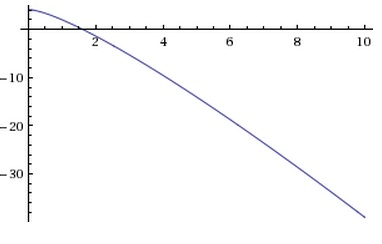
\includegraphics {Funkcja.jpg}\\
1.Dla danych:\\
$a=1$\\
$b=2$\\
$\varepsilon = 0.5$\\
Otrzymujemy :\\
METODA BISEKCJI:\\
f(1.500000)==0.594535\\
f(1.750000)==-0.059616\\
Przyblizone rozwiazanie: f(1.750000)==-0.059616\\
Ilosc krokow: 2\\
METODA NEWTONA:\\
f(1.666667)==0.155841\\
f(1.726606)==0.000632\\
Przyblizone rozwiazanie: f(1.726606)==0.000632\\
2.Dla danych:\\
$a,b$ - takie same jak wyżej \\
$\varepsilon = 0.01$\\
Otrzymujemy :\\
METODA BISEKCJI:\\
f(1.500000)==0.594535\\
f(1.750000)==-0.059616\\
f(1.625000)==0.264492\\
f(1.687500)==0.101752\\
f(1.718750)==0.020903\\
f(1.734375)==-0.019397\\
f(1.726562)==0.000743\\
Przyblizone rozwiazanie: f(1.726562)==0.000743\\
Ilosc krokow: 7\\
METODA NEWTONA:\\
f(1.666667)==0.155841\\
f(1.726606)==0.000632\\
f(1.726850)==0.000000\\
Przyblizone rozwiazanie: f(1.726850)==0.000000\\
Ilosc krokow: 3

\section{Opis Programu}
\subsection{Opis struktur danych oraz funkcji w programie}
Program opiera się w głównej mierze z liczb zmiennoprzeciwnkowych:\\
$x$ określa, czy dana liczba jest większa, równa lub mniejsza od zera\\
$a$ określa dolny przedział przeszukiwań drogą bisekcji\\
$b$ określa górny przedział przeszukiwań drogą bisekcji\\
$epsilon$ określa dokładność przeszukiwań miejsca zerowego\\
Najważniejsze funkcje użyte w programie to:\\
1. Wczytywanie zmiennych a i b\\
2. Sprawdzenie, czy a i b są prawidłowe\\
3. Wczytywanie epsilon oraz sprawdzanie czy jest prawidłowy\\
4. Wypisanie miejsca zerowego metodą bisekcji\\
5. Wypisanie liczby kroków do znalezienia miejsca zerowego\\
6. Wypisanie miejsca zerowego metodą Newtona\\
7. Wypisanie liczby kroków do znalezienia miejsca zerowego\\
\subsection{Opis wejścia-wyjścia}
Program na początku chce otrzymać zmienne $a$ i $b$, które muszą spełniać warunkami opisanymi w punkcie 3.\\
Program będzie sprawdzał, czy podane wartości spełniają warunek. Jeżeli nie, to wyświetli odpowiedni komunikat.\\
Następnie program chce otrzymać wartość $epsilon$, który tak jak powyżej musi spełnić warunek. W przciwnym wypadku wyświetli odpowiedni komunikat.\\
Potem program wypisze miejsce zerowe znalezione metodą bisekcji i Newtona, po każdym znalezionym rozwiązaniu poda ilość kroków potrzebne do znalezienia miejsca zerowego.\\
Po tym wszystkim użytkownik może jeszcze raz podać liczbe $epsilon$, dopóki mu się nie znudzi.\\ 
\subsection{Treść programu}
\begin{lstlisting}
/*Autorzy:
 * Mateusz Miotk
 * Sylwia Kaczmarczyk
 * Michal Kulesz
 * Opis:Program po wczytaniu wartosc a oraz b gdzie 0<a<b
 * oraz podania do "znudzenia" wartosci epsilon
 * bedzie liczyc miejsce zerowe funkcji f(x)=4-2*x-ln x
 * metoda polowienia oraz metoda Newtona.
/********************/

#include <stdio.h>
#include <stdlib.h>
#include <math.h>

/*Nazwa funkcji:sgn(double x)
 * Opis wejscia:liczba x zmiennoprzecinkowa
 * Opis wyjscia:-1 jesli x<0 0 jesli x=0 1 jesli x>0
/****************/
int sgn(double x)
{
    if (x < 0)
	return -1;
    else if (x > 0)
	return 1;
    else
	return 0;
}

/*Funkcja f(x)=4-2*x-ln x*/
double f(double x)
{
    return 4 - 2 * x - log(x);
}

/*Pochodna funkcji f czyli f'(x)=-1/x - 2*/
double f_prim(double x)
{
    return -1 / x - 2;
}

/*Nazwa funkcji:Bisection(double a,double b, double epsilon)
 * Opis wejscia:liczby a,b zmiennoprzecinkowe 
 * okreslajacy badany przedzial
 * Opis funkcji:Funkcja szuka miejsca zerowego metoda bisekcji
 * Opis wyjscia:Kroki i kolejne etapy metody bisekcji
 * Ilosc krokow oraz przyblizone rozwiazanie
/****************/
void Bisection(double a, double b, double epsilon)
{
    unsigned int M = 0;
    double u, v, e, c, w;
    u = f(a);
    v = f(b);
    e = b - a;
    //printf("U==%lf V==%lf e==%lf\n",u,v,e);
    printf("METODA BISEKCJI: \n");
    while (sgn(u) != sgn(v)) {
	M++;
	e /= 2;
	c = a + e;
	w = f(c);
	//printf("KROK %d:f(%lf)==%lf\n", M, c, w);
	if (fabs(w) < epsilon)
	    break;
	//printf("f(%lf)==%lf\n",c,w);
	if (sgn(w) != sgn(u)) {
	    b = c;
	    v = w;
	} else {
	    a = c;
	    u = w;
	}
	//printf("U==%lf V==%lf e==%lf\n",u,v,e);
    }
    printf("Przyblizone rozwiazanie: x==%lf\n", c);
    printf("Ilosc krokow: %d\n", M);
}

/*Nazwa funkcji:Newton(double x_0, double epsilon)
 * Opis wejscia:liczba x_0 zmiennoprzecinkowa oraz epsilon 
 * zmiennoprzecinkowe
 * Opis funkcji:Funkcja szuka miejsca zerowego metoda Newtona
 * Opis wyjscia:Kroki i kolejne etapy metody Newtona
 * Ilosc krokow oraz przyblizone rozwiazanie
/****************/
void Newton(double x_0, double epsilon)
{
    unsigned M = 0;
    double v = f(x_0);
    //printf("f(%lf)==%lf\n",x_0,v);
    printf("METODA NEWTONA: \n");
    double x_1;
    if (fabs(v) < epsilon)
	return;
    while (1) {
	M++;
	x_1 = x_0 - v / f_prim(x_0);
	v = f(x_1);
//	printf("KROK %d:f(%lf)==%lf\n", M, x_1, v);
	if (fabs(x_1 - x_0) <= epsilon) {
	    break;
	}
	x_0 = x_1;
    }
    printf("Przyblizone rozwiazanie: x==%lf\n", x_1);
    printf("Ilosc krokow: %d\n", M);
}

/*Nazwa funkcji:pobranie_danych
 * Opis wejscia:liczby a,b zmiennoprzecinkowe 
 * Opis funkcji:Funkcja wczytuje wartosci a,b i pilnuje poprawnosci
 * danych
 * Opis wyjscia:Wczytane wartosci a i b.
/****************/
void pobranie_danych(double *a, double *b)
{
    printf("Podaj a i b takie ze f(a)*f(b)<0\n");
    while (1) {
	printf("Podaj a: a>0 ");
	scanf("%lf", a);
	while (1) {
	    if ((*a) > 0.0) {
		break;
	    } else {
		printf
	    ("Podales zla wartosc a! a musi byc wieksze od 0\n Podaj a: ");
		scanf("%lf", a);
	    }
	}
	printf("Podaj b: b>a ");
	scanf("%lf", b);
	while (1) {
	    if ((*b) > *a) {
		break;
	    } else {
		printf
	    ("Podales zla wartosc b! b musi byc wieksze od a\n Podaj b: ");
		scanf("%lf", b);
	    }
	}
	if (sgn(f(*a)) != sgn(f(*b))) {
	    break;
	} else {
	    printf
	("Podane a,b nie spelnia wymagania: f(a)*f(b)<0 Podaj inne!\n");
	}
    }
}

void komunikat()
{
    printf
("Program liczy miejsca zerowe funkcji f(x)=4-2*x-ln x\nmetoda polowienia oraz metoda Newtona\n");
}

void policz(double a, double b)
{
    double epsilon;
    printf("Podaj epsilon. 0<epsilon<1 aby zakonczyc:Ctrl+d :");
    while (scanf("%lf", &epsilon) != EOF) {
	if (epsilon > 0 && epsilon < 1) {
	    Bisection(a, b, epsilon);
	    Newton(a, epsilon);
	    printf
		("Podaj nastepna wartosc epsilon. Aby zakonczyc: Ctrl+d :");
	} else {
	    printf("Zla wartosc epsilon! Podaj inna: ");
	}
    }
}

int main()
{
    double a, b;
    komunikat();
    pobranie_danych(&a, &b);
    policz(a, b);
    return EXIT_SUCCESS;
}

\end{lstlisting}
\subsection{Przykładowe wyniki działania programu}
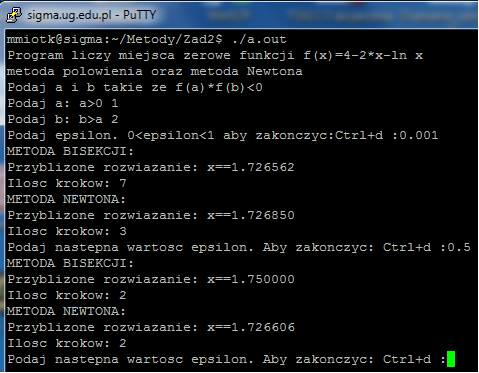
\includegraphics{rozw1.png}\\\\\\\\
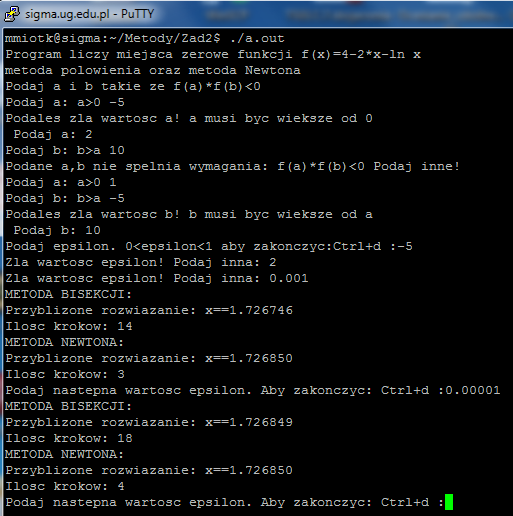
\includegraphics{rozw2.png}
\end{document}